\section{随机平滑与梯度估计}
\label{sec:zo-smoothing}

上一节的估计以原梯度为目标，有限的$h$总带来偏差。于是要问：能否换一个目标，让函数值给出的估计严格无偏？答案是把目标函数在一个小邻域上取平均。平均之后的函数有自己的梯度，而这个梯度恰好可以写成函数值的期望。

打个比方，用原目标比较两点的高低，好比踩着一块小石头判断地面坡度，容易被局部起伏误导；平滑目标则像站在一块平板上，平板的倾斜由它覆盖的整片地面决定。我们估计的是平板的倾斜，不是脚下那一点的坡度。比方的边界也要记住：平板的倾斜和地面的坡度是两个对象，它们的差别要到第~\ref{sec:zo-original-error}节才算清。

\subsection{平滑目标}
\label{sec:zo-smooth-target}

\paragraph{定义}
记$\bm{B}$为$\mathbb{R}^n$中的单位球，即全体长度不超过$1$的向量。下面给出两种平均方式，$\delta>0$是球的半径，$\tau>0$是高斯分布的尺度。

\begin{definition}[球平滑与高斯平滑]
\label{def:zo-smoothing}
设$\bm{v}$在$\bm{B}$上均匀分布，$\bm{w}\sim\mathcal{N}(\bm{0},\bm{I})$。$f$的\term{球平滑}（ball smoothing）与\term{高斯平滑}（Gaussian smoothing）分别是
\begin{equation}
 f^{\mathrm{B}}_{\delta}(\bm{x})=\mathbb{E}_{\bm{v}}\bigl[f(\bm{x}+\delta\bm{v})\bigr],\qquad
 f^{\mathrm{G}}_{\tau}(\bm{x})=\mathbb{E}_{\bm{w}}\bigl[f(\bm{x}+\tau\bm{w})\bigr].
 \label{eq:zo-smoothing}
\end{equation}
前提是期望有定义。它们统称\term{平滑目标}（smoothed objective）。
\end{definition}

\paragraph{定义成立需要什么}
两种平均对$f$的要求不同。球平滑只看$\bm{x}$周围半径$\delta$的球，$f$在这个球上局部可积就够了，比如局部连续。它对球外的$f$没有任何要求。

高斯平滑要看整个空间，于是必须控制$f$在无穷远的增长，局部的好性质帮不上忙。例如$n=1$，$f(x)=e^{x^2}$处处光滑，但
\[
 \mathbb{E}\bigl[e^{(x+\tau w)^2}\bigr]<\infty\quad\Longleftrightarrow\quad 2\tau^2<1.
\]
$\tau\geq1/\sqrt{2}$时高斯平滑根本不存在。多项式增长或指数增长（$\lvert f(\bm{z})\rvert$不超过$Ce^{a\lVert\bm{z}\rVert_2}$）都可以被高斯密度压住。

\paragraph{二次函数上的平滑}
贯穿例上平滑的效果可以算出来。二次函数满足
\[
 f(\bm{x}+\bm{z})=f(\bm{x})+\langle\nabla f(\bm{x}),\bm{z}\rangle+\frac12\bm{z}^\top\bm{H}\bm{z}.
\]
取$\bm{z}$为对称分布的扰动，一次项的期望为零。均匀球上$\mathbb{E}[\bm{v}\bm{v}^\top]=\bm{I}/(n+2)$，所以
\[
 f^{\mathrm{B}}_{\delta}(\bm{x})=f(\bm{x})+\frac{\delta^2\operatorname{tr}\bm{H}}{2(n+2)},\qquad
 f^{\mathrm{G}}_{\tau}(\bm{x})=f(\bm{x})+\frac{\tau^2\operatorname{tr}\bm{H}}{2}.
\]
贯穿例$\operatorname{tr}\bm{H}=10$，$n=2$，分别得到$f+1.25\delta^2$和$f+5\tau^2$。平滑只把目标抬高一个常数，梯度完全不变。所以在二次函数上，平滑目标的梯度就是原梯度，这也解释了上一节的中心差分为什么在二次函数上无偏。

\paragraph{绝对值函数：不可微时平滑仍可微}
平滑真正的用处在不光滑的目标上。$f(x)=\lvert x\rvert$在$0$处没有导数。$n=1$时单位球是区间$[-1,1]$，直接积分得到
\begin{equation}
 f^{\mathrm{B}}_{\delta}(x)=
 \begin{cases}
 \dfrac{x^2+\delta^2}{2\delta},&\lvert x\rvert\leq\delta,\\
 \lvert x\rvert,&\lvert x\rvert>\delta.
 \end{cases}
 \label{eq:zo-abs-ball}
\end{equation}
它的导数在$\lvert x\rvert\leq\delta$上是$x/\delta$，在$x=\pm\delta$处与外侧的$\pm1$衔接，因此连续可微。高斯平滑的结果用误差函数表示：
\[
 f^{\mathrm{G}}_{\tau}(x)=\tau\sqrt{\frac{2}{\pi}}\,e^{-x^2/(2\tau^2)}+x\operatorname{erf}\Bigl(\frac{x}{\sqrt{2}\tau}\Bigr).
\]
图~\ref{fig:zo-smooth-abs}取$\delta=1$，$\tau=1/\sqrt{3}$，这时两种扰动的方差相同。尖点被磨圆了，但代价也在图上：$x=0$处，两条曲线的值分别是$1/2$和约$0.46$，原函数值是$0$。

\begin{BookInlineFigure}
  \centering
  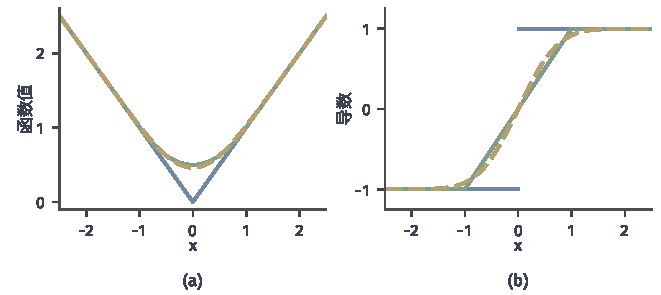
\includegraphics[width=112mm]{figures/05-optimization/05-stochastic-optimization/matplotlib/zo-smooth-abs/figure.pdf}
  \caption{$f(x)=\lvert x\rvert$的平滑。蓝线是原函数，绿线是$\delta=1$的球平滑，黄色虚线是$\tau=1/\sqrt{3}$的高斯平滑。(a)函数值，尖点被磨圆且抬高。(b)导数，原函数在$0$处跳变，平滑后连续。}
  \label{fig:zo-smooth-abs}
\end{BookInlineFigure}

\paragraph{平滑误差}
平滑目标与原目标差多少，由原目标的光滑程度决定。下面的引理后面会多次使用。

\begin{lemma}[平滑的基本性质]
\label{lem:zo-smoothing-properties}
\begin{enumerate}
 \item 若$\nabla f$是$L$-Lipschitz的，则$f^{\mathrm{B}}_{\delta}$与$f^{\mathrm{G}}_{\tau}$的梯度也是$L$-Lipschitz的，并且
 \begin{equation}
  \lvert f^{\mathrm{B}}_{\delta}-f\rvert\leq\frac{L\delta^2}{2},\qquad
  \lVert\nabla f^{\mathrm{B}}_{\delta}-\nabla f\rVert_2\leq L\delta,
  \label{eq:zo-ball-error}
 \end{equation}
 \begin{equation}
  \lvert f^{\mathrm{G}}_{\tau}-f\rvert\leq\frac{L\tau^2n}{2},\qquad
  \lVert\nabla f^{\mathrm{G}}_{\tau}-\nabla f\rVert_2\leq L\tau\sqrt{n}.
  \label{eq:zo-gauss-error}
 \end{equation}
 \item 若$f$是$G$-Lipschitz的，则
 \begin{equation}
  \lvert f^{\mathrm{B}}_{\delta}-f\rvert\leq G\delta.
  \label{eq:zo-lipschitz-error}
 \end{equation}
 \item 若$f$是凸函数，则平滑目标也是凸函数，且$f^{\mathrm{B}}_{\delta}\geq f$，$f^{\mathrm{G}}_{\tau}\geq f$。
\end{enumerate}
\end{lemma}

\begin{proof}
只写球平滑，高斯平滑把$\delta\bm{v}$换成$\tau\bm{w}$，并用$\mathbb{E}\lVert\bm{w}\rVert_2^2=n$与$\mathbb{E}\lVert\bm{w}\rVert_2\leq\sqrt{n}$。

第一项。$\nabla f$连续且至多线性增长，可在期望号下求导：
\[
 \nabla f^{\mathrm{B}}_{\delta}(\bm{x})=\mathbb{E}\bigl[\nabla f(\bm{x}+\delta\bm{v})\bigr].
\]
两点作差，由$\nabla f$的Lipschitz性得到相同常数$L$。由$\mathbb{E}[\bm{v}]=\bm{0}$，
\[
 f^{\mathrm{B}}_{\delta}(\bm{x})-f(\bm{x})=\mathbb{E}\bigl[f(\bm{x}+\delta\bm{v})-f(\bm{x})-\delta\langle\nabla f(\bm{x}),\bm{v}\rangle\bigr].
\]
下降引理给出右端绝对值不超过
\[
 \frac{L}{2}\delta^2\,\mathbb{E}\lVert\bm{v}\rVert_2^2\leq\frac{L\delta^2}{2}.
\]
梯度差由$\nabla f$的Lipschitz性取期望，不超过$L\delta$。

第二项由下式取期望得到：
\[
 \lvert f(\bm{x}+\delta\bm{v})-f(\bm{x})\rvert\leq G\delta\lVert\bm{v}\rVert_2\leq G\delta.
\]

第三项。对每个固定的$\bm{v}$，$\bm{x}\mapsto f(\bm{x}+\delta\bm{v})$是凸函数，凸函数的平均是凸函数。再由Jensen不等式：凸函数在随机点上的平均不小于在平均点上的值，
\[
 f^{\mathrm{B}}_{\delta}(\bm{x})=\mathbb{E}[f(\bm{x}+\delta\bm{v})]\geq f\bigl(\bm{x}+\delta\mathbb{E}[\bm{v}]\bigr)=f(\bm{x}).
\]
\end{proof}

式~\eqref{eq:zo-gauss-error}比式~\eqref{eq:zo-ball-error}多了维数因子。这不是高斯平滑更差，而是$\tau$的含义不同：$\tau\bm{w}$的长度约为$\tau\sqrt{n}$。令$\tau=\delta/\sqrt{n}$时，两组界同阶。

\subsection{单点估计}
\label{sec:zo-one-point}

现在寻找用函数值表示平滑梯度的公式。出发点是一个几何观察，图~\ref{fig:zo-disc-shift}画的是$n=2$的情形。

\paragraph{主要思想}
把球心从$\bm{x}$移动一点点到$\bm{x}+\Delta\bm{x}$，球内积分的变化只发生在边界：右边新进入一片月牙，左边离开一片月牙，中间的部分原封不动。所以球平均的变化率完全由球面上的函数值决定，球内部的值只通过边界起作用。

把这个想法写成式子。月牙在法向$\bm{u}$处的厚度是$\langle\Delta\bm{x},\bm{u}\rangle$，于是积分的一阶变化是球面积分$\int f(\bm{x}+\delta\bm{u})\langle\Delta\bm{x},\bm{u}\rangle\,\mathrm{d}S$。再除以球的体积。半径$\delta$的球面积与球体积之比是$n/\delta$，这就是公式里因子的来历。

\begin{BookInlineFigure}
  \centering
  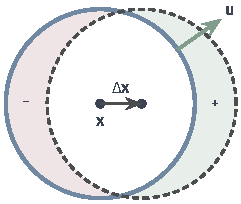
\includegraphics[width=41mm]{figures/05-optimization/05-stochastic-optimization/tikz/zo-disc-shift/figure.pdf}
  \caption{球平滑梯度的来历。蓝色实线是以$\bm{x}$为心的圆，虚线是平移$\Delta\bm{x}$后的圆。绿色月牙是新进入的区域，红色月牙是离开的区域，公共部分对积分的变化没有贡献。月牙在外法向$\bm{u}$处的厚度约为$\langle\Delta\bm{x},\bm{u}\rangle$。}
  \label{fig:zo-disc-shift}
\end{BookInlineFigure}

\begin{theorem}[球平滑的梯度恒等式]
\label{thm:zo-ball-identity}
设$f$在开集$\bm{U}$上连续，闭球$\bm{x}+\delta\bm{B}\subset\bm{U}$，$\bm{u}$在单位球面$\bm{S}$上均匀分布。则$f^{\mathrm{B}}_{\delta}$在$\bm{x}$处可微，且
\begin{equation}
 \nabla f^{\mathrm{B}}_{\delta}(\bm{x})=\frac{n}{\delta}\,\mathbb{E}_{\bm{u}}\bigl[f(\bm{x}+\delta\bm{u})\,\bm{u}\bigr].
 \label{eq:zo-ball-identity}
\end{equation}
\end{theorem}

\begin{proof}
先设$f$连续可微。可在积分号下求导，得
\[
 \partial_if^{\mathrm{B}}_{\delta}(\bm{x})=\frac{1}{\operatorname{vol}(\delta\bm{B})}\int_{\delta\bm{B}}\partial_if(\bm{x}+\bm{z})\,\mathrm{d}\bm{z}.
\]
对向量场$f(\bm{x}+\bm{z})\bm{e}_i$在球$\delta\bm{B}$上用散度定理，外法向是$\bm{z}/\delta$，于是
\[
 \partial_if^{\mathrm{B}}_{\delta}(\bm{x})=\frac{1}{\operatorname{vol}(\delta\bm{B})}\int_{\delta\bm{S}}f(\bm{x}+\bm{z})\frac{z_i}{\delta}\,\mathrm{d}S(\bm{z}).
\]

半径$\delta$的球体积是$c\,\delta^n$，对半径求导得球面积$nc\,\delta^{n-1}$，两者之比为$n/\delta$。把球面积分写成均匀分布下的期望，$\bm{z}=\delta\bm{u}$，就得到式~\eqref{eq:zo-ball-identity}。

再设$f$只连续。取$\bm{x}$的一个小邻域，使它的$\delta$膨胀的闭包是$\bm{U}$内的紧集，用光滑函数$f_k$在这个紧集上一致逼近$f$。$f_k$的平滑函数一致收敛到$f^{\mathrm{B}}_{\delta}$，它们的梯度由恒等式给出，一致收敛到式~\eqref{eq:zo-ball-identity}右端，右端关于位置连续。函数列一致收敛且导数列一致收敛时，极限函数可微且导数等于导数的极限。
\end{proof}

定理要求$f$连续，这个条件不能省。球面在球内的体积为零，把$f$在球面上的值任意修改，$f^{\mathrm{B}}_{\delta}$不变，式~\eqref{eq:zo-ball-identity}的右端却变了。恒等式右端要读取球面上的值，这些值必须与球内的值相联系，连续性保证了这一点。

\paragraph{估计器}
恒等式的右端是期望，抽一个方向就得到它的无偏样本。这称为\term{单点估计}（one-point estimator）：
\begin{equation}
 \hat{\bm{g}}^{(1)}=\frac{n}{\delta}\,y\,\bm{u},\qquad y=f(\bm{x}+\delta\bm{u}).
 \label{eq:zo-one-point}
\end{equation}
它每轮只需一次读数，单点接口也能用。读数含噪声时，只要给定历史、位置和方向时$\zeta$的条件均值为零，噪声项$\zeta\bm{u}$的均值就是零，估计的均值不变，仍是$\nabla f^{\mathrm{B}}_{\delta}(\bm{x})$。注意查询点在球面上，但被估计的是球内平均的梯度，两个集合不要混淆。

\paragraph{常数偏移改变二阶矩}
目标加一个常数$c$，梯度不变，估计的均值也不变，因为$\mathbb{E}[c\bm{u}]=\bm{0}$。可是估计本身变了。由$\lVert\bm{u}\rVert_2=1$，
\begin{equation}
 \mathbb{E}\lVert\hat{\bm{g}}^{(1)}\rVert_2^2=\frac{n^2}{\delta^2}\,\mathbb{E}\bigl[y^2\bigr],
 \label{eq:zo-one-point-moment}
\end{equation}
读数绝对值越大，二阶矩越大，哪怕它的大小与优化毫无关系。

贯穿例起点$f=45$，取$\delta=0.1$，$n=2$，因子$n/\delta=20$。沿$\pm\bm{e}_1$方向的两个估计是
\[
 \bm{u}=\bm{e}_1:\ (918.1,\ 0),\qquad\bm{u}=-\bm{e}_1:\ (-882.1,\ 0).
\]
沿$\pm\bm{e}_2$方向是
\[
 \bm{u}=\bm{e}_2:\ (0,\ 918.9),\qquad\bm{u}=-\bm{e}_2:\ (0,\ -882.9).
\]
四个向量的平均是$(9,9)$，等于真实梯度，但每个向量的长度约为$900$，比梯度长度$12.7$大七十倍。巨大的数相互抵消后才剩下需要的信号，如图~\ref{fig:zo-single-cloud}(a)。

如果事先知道$f$大约在$45$附近，把估计中的$y$换成$y-45$，均值不变，散布却缩回$20$左右，如图~\ref{fig:zo-single-cloud}(b)。可是这个常数算法事先并不知道，这就引出了下一小节的成对读数。

\begin{BookInlineFigure}
  \centering
  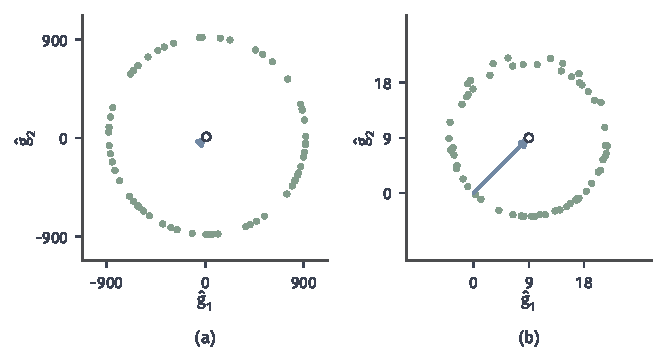
\includegraphics[width=112mm]{figures/05-optimization/05-stochastic-optimization/matplotlib/zo-single-cloud/figure.pdf}
  \caption{贯穿例起点的单点估计，$\delta=0.1$，$60$个随机方向。绿点是估计值，蓝色箭头是真实梯度$(9,9)$，空心圆是它的终点。(a)原读数的估计分布在半径约$900$的圆上，比梯度大两个量级。(b)读数减去常数$45$后，同样的$60$个方向给出的估计缩到半径约$13$的圆上。两张图的坐标范围不同。}
  \label{fig:zo-single-cloud}
\end{BookInlineFigure}

\paragraph{平滑目标的光滑常数}
单点估计常用于$f$只是$G$-Lipschitz的情形。这时$f^{\mathrm{B}}_{\delta}$是否光滑？由恒等式~\eqref{eq:zo-ball-identity}，对任意$\bm{x},\bm{z}$，
\[
 \lVert\nabla f^{\mathrm{B}}_{\delta}(\bm{x})-\nabla f^{\mathrm{B}}_{\delta}(\bm{z})\rVert_2
 \leq\frac{n}{\delta}\mathbb{E}\lvert f(\bm{x}+\delta\bm{u})-f(\bm{z}+\delta\bm{u})\rvert
 \leq\frac{nG}{\delta}\lVert\bm{x}-\bm{z}\rVert_2.
\]
所以$f^{\mathrm{B}}_{\delta}$的光滑常数不超过$nG/\delta$。$\delta$越小，平滑目标越接近原目标，但也越弯曲。这个上界不一定紧，它的作用是说明平滑后有光滑常数可用。

\subsection{双点估计}
\label{sec:zo-two-point}

成对查询允许把单点估计里的大数减掉。在相反方向各读一次，得到\term{双点估计}（two-point estimator）：
\begin{equation}
 \hat{\bm{g}}^{(2)}=\frac{n}{2\delta}\bigl(y_+-y_-\bigr)\bm{u},\qquad
 y_\pm=f(\bm{x}\pm\delta\bm{u}).
 \label{eq:zo-two-point}
\end{equation}
这正是第~\ref{sec:zo-random-direction}节的式~\eqref{eq:zo-random-direction}取$h=\delta$。公式相同，这里的解释却更精确。

\paragraph{为什么均值是平滑梯度}
$\bm{u}$和$-\bm{u}$同分布，所以单点估计用$-\bm{u}$代替$\bm{u}$，期望不变：
\[
 \frac{n}{\delta}\mathbb{E}\bigl[f(\bm{x}+\delta\bm{u})\bm{u}\bigr]
 =\frac{n}{\delta}\mathbb{E}\bigl[f(\bm{x}-\delta\bm{u})(-\bm{u})\bigr].
\]
两式相加除以$2$，右端正是$\mathbb{E}[\hat{\bm{g}}^{(2)}]$，左端由恒等式等于$\nabla f^{\mathrm{B}}_{\delta}(\bm{x})$。于是
\begin{equation}
 \mathbb{E}\bigl[\hat{\bm{g}}^{(2)}\bigr]=\nabla f^{\mathrm{B}}_{\delta}(\bm{x}).
 \label{eq:zo-two-point-mean}
\end{equation}

把两节的说法对照起来，同一个向量有两种读法。作为原梯度的近似，它有偏差，Hessian是Lipschitz时偏差是$O(\delta^2)$；作为平滑梯度的估计，它严格无偏。表~\ref{tab:zo-two-views}列出两种读法的差别。选哪种读法，取决于最终想回答关于哪个目标的问题。

\begin{BookInlineTable}
  \centering
  \begin{tabular}{@{}lll@{}}
    \toprule
    读法 & 估计对象 & 偏差\\
    \midrule
    有限差分 & $\nabla f(\bm{x})$ & 一般非零，随$\delta$缩小\\
    平滑估计 & $\nabla f^{\mathrm{B}}_{\delta}(\bm{x})$ & 严格为零\\
    \bottomrule
  \end{tabular}
  \caption{同一个双点向量的两种读法。原目标不可微时第一种读法没有对象，第二种仍然成立。}
  \label{tab:zo-two-views}
\end{BookInlineTable}

\paragraph{减去中心值的形式}
另一个双点形式把$y_-$换成中心读数：
\begin{equation}
 \hat{\bm{g}}^{(\mathrm{c})}=\frac{n}{\delta}\bigl(f(\bm{x}+\delta\bm{u})-f(\bm{x})\bigr)\bm{u}.
 \label{eq:zo-center-point}
\end{equation}
由$\mathbb{E}[f(\bm{x})\bm{u}]=\bm{0}$，它的均值也是$\nabla f^{\mathrm{B}}_{\delta}(\bm{x})$。两种形式都消除了常数偏移，贯穿例上把“很大的$45$”去掉了。

\paragraph{二阶矩的比较}
消去偏移后，估计的大小由差商决定。下面的引理针对光滑目标给出统一的界。

\begin{lemma}[双点估计的二阶矩]
\label{lem:zo-two-point-moment}
设$\nabla f$是$L$-Lipschitz的，读数精确。对估计~\eqref{eq:zo-two-point}和~\eqref{eq:zo-center-point}，都有
\begin{equation}
 \mathbb{E}\lVert\hat{\bm{g}}\rVert_2^2\leq 2n\lVert\nabla f(\bm{x})\rVert_2^2+\frac{n^2L^2\delta^2}{2}.
 \label{eq:zo-two-point-moment}
\end{equation}
\end{lemma}

\begin{proof}
记$\bm{g}=\nabla f(\bm{x})$，$\hat{\bm{g}}=nD\bm{u}$，其中$D$是对应的差商，写成$D=\langle\bm{g},\bm{u}\rangle+r$。由式~\eqref{eq:zo-central-L}或下降引理，两种形式都有$\lvert r\rvert\leq L\delta/2$。

用$(a+b)^2\leq2a^2+2b^2$和$\lVert\bm{u}\rVert_2=1$，
\[
 \lVert\hat{\bm{g}}\rVert_2^2=n^2D^2\leq 2n^2\langle\bm{g},\bm{u}\rangle^2+\frac{n^2L^2\delta^2}{2}.
\]
取期望，再用$\mathbb{E}[\bm{u}\bm{u}^\top]=\bm{I}/n$，得到结论。
\end{proof}

式~\eqref{eq:zo-two-point-moment}与单点的式~\eqref{eq:zo-one-point-moment}对比，分母里的$\delta^2$不见了，$\delta$可以取得很小而不使估计爆炸。这是精确读数下成对查询的实质收益。

两种双点形式的差别要看函数。贯穿例上，对称形式的差商精确等于方向导数，二阶矩是$n\lVert\bm{g}\rVert_2^2$；中心形式多出$\tfrac{\delta}{2}\bm{u}^\top\bm{H}\bm{u}$，二阶矩更大。在极小点$\bm{g}=\bm{0}$处，对称形式的估计恒为零，而中心形式不为零，这点上对称形式完全不抖动。$f=\lvert x\rvert$在$x=0$处，对称形式同样恒为零，中心形式的估计是$\pm1$。

但是“方差改善”不是无条件的结论。第一，改善来自消去$f$的大小，如果$f$本身在零附近，单点估计并没有这部分额外的方差。第二，带独立噪声时，两次单点估计取平均与一次双点估计噪声贡献相同，都是$n^2\sigma^2/(2\delta^2)$，第~\ref{sec:zo-pair-noise}节会算出来。所以成对读数消去的是函数值的公共部分，不是噪声。

\subsection{高斯方向估计}
\label{sec:zo-gaussian}

球面方向需要扰动恰好落在半径$\delta$的球面上。如果改用高斯扰动，查询点不再被限制在球面上，分析也更简单，因为高斯密度的导数有封闭形式。

\paragraph{主要思想}
作变量替换$\bm{z}=\bm{x}+\tau\bm{w}$，把高斯平滑写成
\[
 f^{\mathrm{G}}_{\tau}(\bm{x})=\frac{1}{(2\pi\tau^2)^{n/2}}\int f(\bm{z})\exp\Bigl(-\frac{\lVert\bm{z}-\bm{x}\rVert_2^2}{2\tau^2}\Bigr)\mathrm{d}\bm{z}.
\]
现在$\bm{x}$只出现在指数里，$f$不必可微，梯度全部落到光滑的高斯核上。这与球平滑的情况类似：导数从$f$转移到了平均方式上。

\begin{theorem}[高斯平滑的梯度恒等式]
\label{thm:zo-gauss-identity}
设$f$可测，存在$C,a\geq0$使$\lvert f(\bm{z})\rvert$处处不超过$Ce^{a\lVert\bm{z}\rVert_2}$，$\bm{w}\sim\mathcal{N}(\bm{0},\bm{I})$。则$f^{\mathrm{G}}_{\tau}$可微，且
\begin{equation}
 \nabla f^{\mathrm{G}}_{\tau}(\bm{x})=\frac{1}{\tau}\,\mathbb{E}_{\bm{w}}\bigl[f(\bm{x}+\tau\bm{w})\,\bm{w}\bigr].
 \label{eq:zo-gauss-identity}
\end{equation}
\end{theorem}

\begin{proof}
高斯核对$\bm{x}$的梯度等于核本身乘$(\bm{z}-\bm{x})/\tau^2$。当$\bm{x}$在一个有界邻域内时，被积函数对$\bm{x}$的梯度被一个不依赖$\bm{x}$的可积函数控制：指数增长被高斯衰减压住。由控制收敛定理，可在积分号下求导，得
\[
 \nabla f^{\mathrm{G}}_{\tau}(\bm{x})=\frac{1}{(2\pi\tau^2)^{n/2}}\int f(\bm{z})\frac{\bm{z}-\bm{x}}{\tau^2}\exp\Bigl(-\frac{\lVert\bm{z}-\bm{x}\rVert_2^2}{2\tau^2}\Bigr)\mathrm{d}\bm{z}.
\]
再换回$\bm{z}=\bm{x}+\tau\bm{w}$，$(\bm{z}-\bm{x})/\tau^2=\bm{w}/\tau$，即得结论。
\end{proof}

这个定理比球面的恒等式要求的局部性质弱：$f$可以不连续，因为积分覆盖整个空间，$f$在零测集上的值不起作用。要求转移到了全局的增长上，这正好是定义中高斯平滑存在所需要的。

\paragraph{三种形式}
抽一个$\bm{w}$，式~\eqref{eq:zo-gauss-identity}给出单点形式。与球面的情形一样，减去中心值或取对称差，均值不变：
\begin{equation}
 \hat{\bm{g}}^{\mathrm{G}}=\frac{y}{\tau}\bm{w},\qquad
 \hat{\bm{g}}^{\mathrm{Gc}}=\frac{y-f(\bm{x})}{\tau}\bm{w},\qquad
 \hat{\bm{g}}^{\mathrm{Gs}}=\frac{y-y'}{2\tau}\bm{w},
 \label{eq:zo-gauss-estimators}
\end{equation}
其中$y=f(\bm{x}+\tau\bm{w})$，$y'=f(\bm{x}-\tau\bm{w})$。第二种利用了$\mathbb{E}[\bm{w}]=\bm{0}$，第三种利用了$\bm{w}$与$-\bm{w}$同分布。

贯穿例起点，取$\tau=0.1$，抽到$\bm{w}=(1,-0.5)$。对称形式的读数和差商是
\[
 f(9.1,0.95)=45.46625,\qquad f(8.9,1.05)=44.56625,\qquad\frac{y-y'}{2\tau}=4.5.
\]
这里$\langle\nabla f,\bm{w}\rangle=9-4.5=4.5$，吻合。估计是$4.5\,\bm{w}=(4.5,-2.25)$。

\paragraph{与球面方向的区别}
公式里没有因子$n$，这是因为$\mathbb{E}[\bm{w}\bm{w}^\top]=\bm{I}$，球面方向则是$\bm{I}/n$。如果把球面的归一化照搬过来写成$(n/\tau)y\bm{w}$，二次函数上的均值就变成$n\nabla f$，整整放大$n$倍。

另一个区别是扰动的长度。$\lVert\bm{w}\rVert_2$是随机的，大约是$\sqrt{n}$，如图~\ref{fig:zo-sphere-gauss}(b)。$\tau$只是尺度，不是查询半径。$n=2$时
\[
 \mathbb{P}\bigl(\lVert\bm{w}\rVert_2>3\bigr)=e^{-4.5}\approx0.011,
\]
一百次里约有一次偏离三个尺度。要与球面半径$\delta$对应，应取$\tau=\delta/\sqrt{n}$，这时$\tau\bm{w}$的均方长度等于$\delta^2$。

\begin{BookInlineFigure}
  \centering
  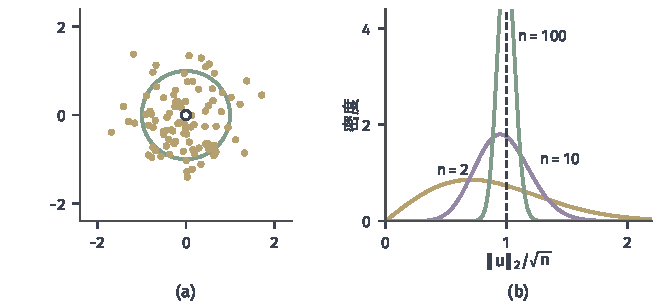
\includegraphics[width=112mm]{figures/05-optimization/05-stochastic-optimization/matplotlib/zo-sphere-gauss/figure.pdf}
  \caption{球面方向与高斯方向。(a)$n=2$，绿圆是半径$\delta=1$的球面查询位置，黄点是尺度$\tau=1/\sqrt{2}$的高斯查询点，二者均方长度相同，高斯点散布在圆内外。(b)$\lVert\bm{w}\rVert_2/\sqrt{n}$的密度。维数增大时高斯方向的长度集中到$\sqrt{n}$附近，$n=2$时差异很大。}
  \label{fig:zo-sphere-gauss}
\end{BookInlineFigure}

二次函数上，对称形式的二阶矩可以直接算：
\[
 \mathbb{E}\bigl[\langle\bm{g},\bm{w}\rangle^2\lVert\bm{w}\rVert_2^2\bigr]=(n+2)\lVert\bm{g}\rVert_2^2.
\]
所以方差是$(n+1)\lVert\bm{g}\rVert_2^2$，比球面方向的$(n-1)\lVert\bm{g}\rVert_2^2$略大，多出来的部分来自长度的波动。一般光滑函数上有类似的上界：
\begin{equation}
 \mathbb{E}\lVert\hat{\bm{g}}^{\mathrm{Gs}}\rVert_2^2\leq2(n+2)\lVert\nabla f(\bm{x})\rVert_2^2+\frac{L^2\tau^2}{2}n(n+2)(n+4).
 \label{eq:zo-gauss-moment}
\end{equation}
推导与引理~\ref{lem:zo-two-point-moment}相同，只是余项是$\lvert r\rvert\leq L\tau\lVert\bm{w}\rVert_2^2/2$，再用高斯矩$\mathbb{E}\lVert\bm{w}\rVert_2^6=n(n+2)(n+4)$。

\subsection{成对读数的噪声}
\label{sec:zo-pair-noise}

到此为止的二阶矩都假设读数精确。本小节回到第~\ref{sec:zo-pair-interface}节的接口问题：读数含噪声时，成对差分的波动是多少？

\paragraph{独立噪声}
采用式~\eqref{eq:zo-independent-pair}，$\zeta_+,\zeta_-$条件独立，均值零，方差不超过$\sigma^2$。差商的噪声部分是$(\zeta_+-\zeta_-)/(2\delta)$，于是
\begin{equation}
 \operatorname{Var}\Bigl(\frac{\zeta_+-\zeta_-}{2\delta}\Bigr)\leq\frac{\sigma^2}{2\delta^2}.
 \label{eq:zo-independent-variance}
\end{equation}
半径减半，方差变成四倍。噪声大小不随距离变小，分母却在变小。图~\ref{fig:zo-pair-noise}中黄线的斜率是$-2$。

噪声与差商主项的交叉项为零，因为噪声的条件均值是零。代入估计，$\lVert\hat{\bm{g}}^{(2)}\rVert_2^2$的期望增加$n^2\sigma^2/(2\delta^2)$。结合引理~\ref{lem:zo-two-point-moment}，得到后面反复使用的二阶矩界：
\begin{equation}
 \mathbb{E}\lVert\hat{\bm{g}}^{(2)}\rVert_2^2\leq2n\lVert\nabla f(\bm{x})\rVert_2^2+V,\qquad
 V=\frac{n^2L^2\delta^2}{2}+\frac{n^2\sigma^2}{2\delta^2}.
 \label{eq:zo-noisy-moment}
\end{equation}

\paragraph{单点平均与成对差分}
单点估计用两次独立读数和两个独立方向取平均时，噪声贡献是
\[
 \frac14\Bigl(\frac{n^2\sigma^2}{\delta^2}+\frac{n^2\sigma^2}{\delta^2}\Bigr)=\frac{n^2\sigma^2}{2\delta^2},
\]
与双点估计完全相同。这验证了前面的说法：独立噪声下，配对不减少噪声，只消去函数值的公共部分。

\paragraph{共享样本}
采用式~\eqref{eq:zo-shared-pair}，差分的方差包含协方差：
\begin{equation}
 \operatorname{Var}\bigl[F(\bm{q}_+;\bm{\xi})-F(\bm{q}_-;\bm{\xi})\bigr]
 =\operatorname{Var}F_++\operatorname{Var}F_--2\operatorname{Cov}(F_+,F_-).
 \label{eq:zo-shared-variance}
\end{equation}
共享样本带来的是正的协方差，协方差越大，抵消越多。若两个噪声的相关系数是$\rho$且方差都是$\sigma^2$，差的方差是$2\sigma^2(1-\rho)$，从$\rho=0$的独立到$\rho=1$的完全抵消，中间是连续变化的。

\paragraph{三个例子}
共享样本的效果取决于样本函数本身的波动。

第一个例子是两点共享同一个加性噪声，$F(\bm{x};\xi)=f(\bm{x})+\xi$。差分时$\xi$完全消失，噪声方差为零，无论半径多小，差商都是精确的。

第二个例子是样本函数关于$\bm{x}$Lipschitz，比如$F(\bm{x};\bm{\xi})=f(\bm{x})+\bm{\xi}^\top\bm{x}$。差分的随机部分是
\[
 \frac{\bm{\xi}^\top(\bm{q}_+-\bm{q}_-)}{2\delta}=\bm{\xi}^\top\bm{u},
\]
它不依赖$\delta$。一般地，若$F(\cdot;\bm{\xi})$是Lipschitz的，常数为$G(\bm{\xi})$，差商的二阶矩不超过$\mathbb{E}[G(\bm{\xi})^2]$，$\delta$可以取得很小。图~\ref{fig:zo-pair-noise}中绿线是水平的。

第三个例子是样本函数不连续。$F(x;\xi)=\mathbb{1}\{x>\xi\}$，$\xi$的密度为$p$。共享$\xi$时差分只在$\xi\in[x-h,x+h)$时非零，概率约$2hp(x)$，于是差商方差约为
\[
 \frac{2hp(x)}{4h^2}=\frac{p(x)}{2h}.
\]
它比独立噪声的$1/h^2$好，但仍随$h$缩小而增大，图~\ref{fig:zo-pair-noise}中紫线的斜率是$-1$。所以共享样本带来改善的前提是差值的波动受控，只说“用了同一个种子”并不够。

\begin{BookInlineFigure}
  \centering
  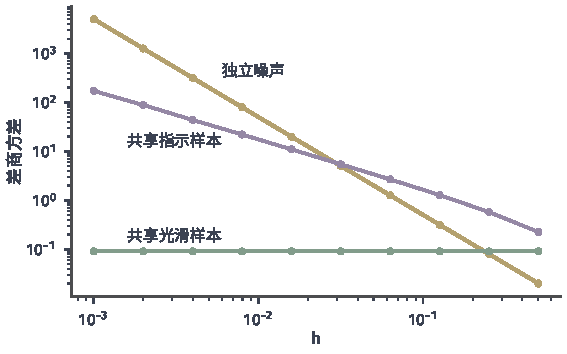
\includegraphics[width=96mm]{figures/05-optimization/05-stochastic-optimization/matplotlib/zo-pair-noise/figure.pdf}
  \caption{中心差商的方差随$h$的变化，$x=0.5$。黄线：独立加性噪声，标准差$0.1$，斜率$-2$。紫线：共享指示样本$F=\mathbb{1}\{x>\xi\}$，$\xi\sim\mathcal{N}(0,1)$，斜率$-1$。绿线：共享光滑样本$F=x^2/2+\xi x$，$\xi$标准差$0.3$，方差不随$h$变化。共享同一加性噪声时方差为零，未画出。每点来自$4\times10^6$次模拟。}
  \label{fig:zo-pair-noise}
\end{BookInlineFigure}
